\documentclass[tikz]{standalone}
\usepackage{tikz}
\usepackage{pgfplots,graphicx}
\pgfplotsset{compat=newest,compat/show suggested version=false}
\usetikzlibrary{pgfplots.groupplots,matrix}
\usetikzlibrary{positioning,fit,calc,shapes,patterns,automata}
\usepackage{tabularx,xfrac,color,makecell}
\usepackage{array}
\usetikzlibrary{plotmarks}
\usepackage{aurical}
\usepackage[T1]{fontenc}

\usepackage{fontspec}
\setmainfont{Aozora Mincho Regular}

\newcommand{\lmr}{\fontfamily{lmr}\selectfont} % Latin Modern Roman

\tikzset
	{
		tag/.style=
			{
				font=\footnotesize,
				anchor=north west,
				outer sep=0,
				rectangle
			}	
	}
\tikzset
	{
		pron/.style=
			{
				font=\scriptsize,
				anchor=south west,
				outer sep=0,
				draw,
				rectangle,
				ultra thin
			}	
	}
\newcommand{\vier}[4]
	{
		\begin{tabular}{@{}r@{}c@{  }l@{}}
			\textsc{\textbf{\color{red}{#1}}} & $\mathbf{\wr}$ & \textbf{\color{blue}{#2}} \\
			\textsc{#3} & $\wr$ & #4
		\end{tabular}
	}
\begin{document}
\begin{tikzpicture}
\matrix (m) 
	[
		matrix of nodes,
		nodes=
			{
				draw,
				rectangle,
				ultra thick,
				outer sep=0,
				anchor=center,
				minimum height=5cm,minimum width=4cm
			}
	]
	{
		{
\includegraphics[width=4cm]{capital.pdf}} &
		{
\includegraphics[width=4cm]{see.pdf}} &
		{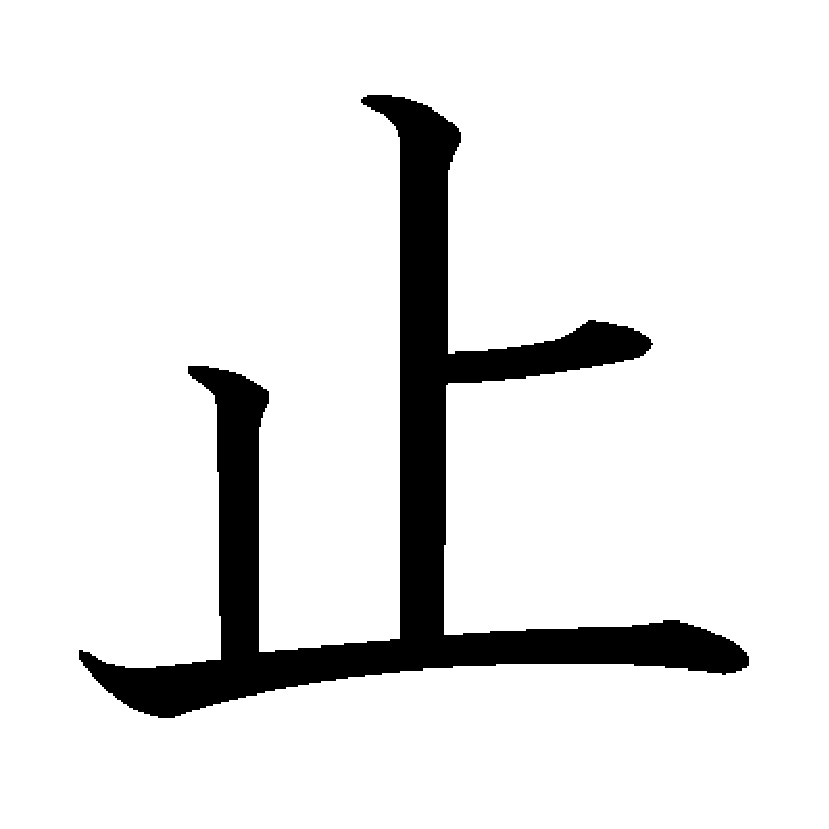
\includegraphics[width=4cm]{stop.pdf}} &
		{
\includegraphics[width=4cm]{seven.pdf}} \\
		{
\includegraphics[width=4cm]{few.pdf}} &
		{
\includegraphics[width=4cm]{south.pdf}} &
		{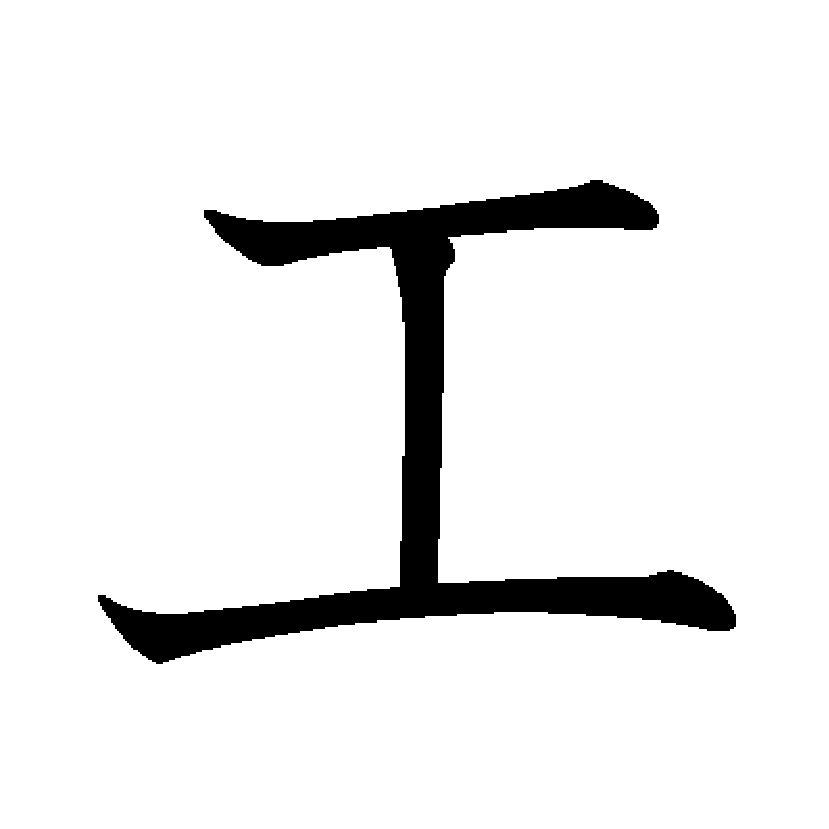
\includegraphics[width=4cm]{craft.pdf}} &
		{
\includegraphics[width=4cm]{left.pdf}} \\
		{
\includegraphics[width=4cm]{tall.pdf}} &
		{
\includegraphics[width=4cm]{buy.pdf}} &
		{
\includegraphics[width=4cm]{hundred.pdf}} &
		{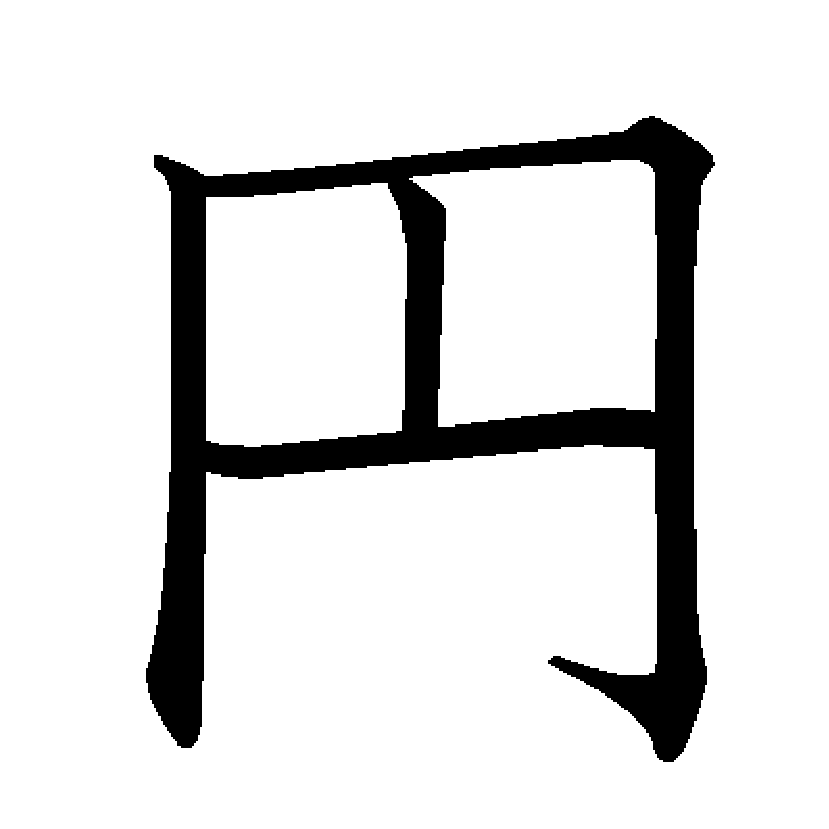
\includegraphics[width=4cm]{circle.pdf}} \\
		{
\includegraphics[width=4cm]{basis.pdf}} &
		{
\includegraphics[width=4cm]{neck.pdf}} &
		{
\includegraphics[width=4cm]{walk.pdf}} &
		{
\includegraphics[width=4cm]{child.pdf}} \\
		{
\includegraphics[width=4cm]{like.pdf}} &
		{
\includegraphics[width=4cm]{old.pdf}} &
		{
\includegraphics[width=4cm]{fire.pdf}} &
		{
\includegraphics[width=4cm]{winter.pdf}} \\
	};
\node [tag] at (m-1-1.north west) {\Fontlukas Capital};
\node [tag] at (m-1-2.north west) {\Fontlukas See};
\node [tag] at (m-1-3.north west) {\Fontlukas Stop};
\node [tag] at (m-1-4.north west) {\Fontlukas Seven};
\node [tag] at (m-2-1.north west) {\Fontlukas Few};
\node [tag] at (m-2-2.north west) {\Fontlukas South};
\node [tag] at (m-2-3.north west) {\Fontlukas Craft};
\node [tag] at (m-2-4.north west) {\Fontlukas Left};
\node [tag] at (m-3-1.north west) {\Fontlukas Tall};
\node [tag] at (m-3-2.north west) {\Fontlukas Buy};
\node [tag] at (m-3-3.north west) {\Fontlukas Hundred};
\node [tag] at (m-3-4.north west) {\Fontlukas Circle};
\node [tag] at (m-4-1.north west) {\Fontlukas Basis};
\node [tag] at (m-4-2.north west) {\Fontlukas Neck};
\node [tag] at (m-4-3.north west) {\Fontlukas Walk};
\node [tag] at (m-4-4.north west) {\Fontlukas Child};
\node [tag] at (m-5-1.north west) {\Fontlukas Like};
\node [tag] at (m-5-2.north west) {\Fontlukas Old};
\node [tag] at (m-5-3.north west) {\Fontlukas Fire};
\node [tag] at (m-5-4.north west) {\Fontlukas Winter};

\node [pron] at (m-1-1.south west) {\vier{キョウ}{--}{ケイ}{--}};
\node [pron] at (m-1-2.south west) {\vier{ケン}{み}{--}{--}};
\node [pron] at (m-1-3.south west) {\vier{シ}{と}{--}{--}};
\node [pron] at (m-1-4.south west) {\vier{シチ}{なな}{--}{なの}};
\node [pron] at (m-2-1.south west) {\vier{ショウ}{すく; すこ}{--}{--}};
\node [pron] at (m-2-2.south west) {\vier{ナン}{みなみ}{--}{--}};
\node [pron] at (m-2-3.south west) {\vier{コウ}{--}{ク}{--}};
\node [pron] at (m-2-4.south west) {\vier{--}{ひだり}{サ}{--}};
\node [pron] at (m-3-1.south west) {\vier{コウ}{たか}{--}{--}};
\node [pron] at (m-3-2.south west) {\vier{--}{か}{バイ}{--}};
\node [pron] at (m-3-3.south west) {\vier{ヒャク}{--}{--}{--}};
\node [pron] at (m-3-4.south west) {\vier{エン}{まる}{--}{--}};
\node [pron] at (m-4-1.south west) {\vier{ゲン; ガン}{もと}{--}{--}};
\node [pron] at (m-4-2.south west) {\vier{シュ}{くび}{--}{--}};
\node [pron] at (m-4-3.south west) {\vier{ホ}{ある}{--}{--}};
\node [pron] at (m-4-4.south west) {\vier{シ}{こ}{ス}{--}};
\node [pron] at (m-5-1.south west) {\vier{コウ}{すき}{--}{この}};
\node [pron] at (m-5-2.south west) {\vier{コ}{ふる}{--}{--}};
\node [pron] at (m-5-3.south west) {\vier{カ}{ひ}{--}{--}};
\node [pron] at (m-5-4.south west) {\vier{トウ}{ふゆ}{--}{--}};

\node (webs)
	[
		anchor=south east,
		color=lightgray,
		outer sep=0
	]
		at (m.north east)
	{
		http:{/}{/}kanji.nihongo.cz/home
	};
\node (chap)
	[
		anchor=south west,
		color=black,
		outer sep=0,
		font=\huge
	]
		at (m.north west)
	{
		\textbf{\lmr Chapter 3}
	};
\end{tikzpicture}
\end{document}